\chapter{Kestrel}
\label{chap:Kestrel} 

Many-Task Computing (MTC) applications span a broad range of possible
configurations, but utilizing “large num- bers of computing resources over
short periods of time to accomplish many computational tasks, where the primary
metrics are in seconds” [1] is one of the emphasized aspects. Marshalling
and releasing computational resources with the temporal granularity needed for
such applications is prob- lematic on the grid and in overlays such as Virtual
Organi- zation Clusters (VOC) [2, 3] where compute nodes can be created and
destroyed on demand. Kestrel is designed to explore methods of creating a fault-
tolerant, scalable, and cross-platform job scheduling system for heterogeneous,
intermittently connected compute nodes. Kestrel addresses the problem posed
by interrupted connec- tivity of both computing agents and user agents by
building on the Extensible Messaging and Presence Protocol (XMPP) [4, 5]. The
presence notification system provided by XMPP allows Kestrel manager nodes to
track resource availability in the compute node pool in real time. Kestrel can
immedi- ately remove computing node from a list of available nodes, preventing
the scheduling of jobs on nonexistent machines. Other intermittently connected
agents do not necessarily have to be of a computational nature. For example, a
small swarm of robotic agents with network capabilities could be joined in a
resource pool where scheduled jobs are physi- cal actions to be performed. The
scale of current instant messaging systems indicates that an XMPP based frame-
work would allow for the creation of extremely large pools of heterogeneous
agents for real-time computing. The cross- platform criterion is achieved by
implementing the system in Python [6] using the SleekXMPP [7] library.


Started in the summer of 2009, Kestrel is a job scheduling system
based on the Extensible Messaging and Presence Protocol, or XMPP
\cite{RFC3920,RFC3921}. The original environment for
which Kestrel was designed to manage was disparate collections of virtual
machines pooled together into a single cluster, or a Virtual Organization
Cluster (VOC) \cite{Murphy2009} as shown in figure \ref{fig:Kestrel-Arch}.
However, compute nodes in VOCs are temporary and can be created and destroyed
on demand, or the virtual machines may be killed by the hosting resource
provider without warning. XMPP provides a solution for managing heterogeneous,
intermittently connecting compute elements through the use of service discovery
and presence notifications; Kestrel builds on these features with XMPP
sub-protocols for requesting and dispatching tasks in such a cloud environment.


\section{Architecture}
Based upon the traditional master-worker architecture, a Kestrel pool is made
from four classes of agents: clients, workers, managers, and servers. Logically,
the client, worker, and manager entities form a star network, with a manager as
the hub; however, since XMPP is used, the actual topology will look as described
in section \ref{sec:The-XMPP-Network}. It is possible for multiple entities to
reside on the same physical or virtual machine. Since all agents connect to an
XMPP server for routing communications instead of connecting directly to each
other, the issues of NAT traversal are eliminated; the result is an overlay
network that allows agents to communicate freely irrespective of the underlying
networking setup, whether on physical or virtual machines.

\begin{figure}
\caption{The logical network communication paths for a Kestrel pool. Messages
may be routed through at most two XMPP servers for any of the paths shown.}
\end{figure}

\subsection{Well-Known JIDs}
Since the Kestrel manager is an XMPP component, it may be addressed by many JIDs
with different username portions. For example, the JIDs \texttt{pool@manager.example.org}
and \texttt{job\_42@manager.example.org} will both be delivered to the Kestrel
manager. Kestrel reserves two particular usernames for interaction with clients
and workers. The first is \texttt{submit} which may accept job submissions and
status requests from clients. The second is \texttt{pool} which is contacted
by workers attempting to join the pool, and by clients requesting the pool's
status.

Each job accepted by the manager is also given a unique JID username of
the form: \texttt{job\_\#}, where the \texttt{\#} is replaced by the
job's ID value. For example, a job with an ID of 37 may be referenced as
\texttt{job\_37@manager.example.org}. Each job submitted to Kestrel may
be composed of multiple ``tasks'', which are the individual instances
of the job's command to execute. The resource portion of a job's JID
refers to a particular task, e.g. a worker receiving a task from the JID
\texttt{job\_37@manager.example.org/99} knows that it is executing task 99 from
job 37. Once a job has been accepted by the manager, a subscription request is
made from the job's JID to the client's JID, allowing the user to easily monitor
the status of the job from an IM client as shown in figure \ref{fig:IM-Client}

\begin{figure}
\begin{centering}
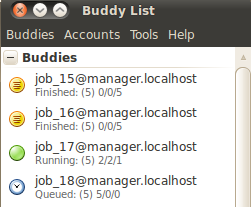
\includegraphics[width=6cm]{figures/im_client}
\end{centering}
\caption{\label{fig:IM-Client} Monitoring job statuses through a normal instant
messaging client. Once accepted by the manager, jobs request to be
added to the user's roster to deliver current status updates. Running
jobs display themselves as available while queued jobs are displayed
as away. For finished jobs, an extended away status is shown. The
status message for each job includes a sequence of four numbers indicating,
in order, the number of tasks requested, queued, running, and completed.
Jobs may be canceled from an IM client by removing it from the roster.}
\end{figure}

\section{Clients}
Client agents are used by end users for submitting and managing jobs. As such,
a client implementation can be a minimal XMPP client with just the logic needed
to submit jobs and status requests, but more full-featured and existing clients
such as Pidgin \cite{Pidgin} or GTalk \cite{GTalk} can also be used. As part of
the typical use case, using the client implementation supplied with Kestrel,
client agents join the system intermittently and for just long enough to send a
single command to the manager and receive a response. Clients that remain connected
will receive presence subscription requests from JIDs representing the user's jobs,
which send status updates as tasks are dispatched or completed, allowing for 
continuous status monitoring.

\subsection{Job Management}
\label{sec:Job-Management} 
Creating and monitoring jobs can now
be carried out through the command line instead of having to rely
upon an instant messaging client such as Pidgin \cite{Pidgin} or
Adium \cite{Adium}. However, as shown in figure \ref{fig:IM-Client},
important job status information can be received through a client
program as part of the job JID's presence status updates, such as
the number of queued, running, and completed tasks. Jobs that are
accepted, and assigned a JID, may be added to the user's XMPP roster
(also referred to as a buddy list in other messaging systems). Removing
the job from the roster will cancel the job and terminate running
tasks. From the command line, jobs may be submitted, canceled, and
queried for their current status using the commands shown in figure
\ref{fig:Commands}.

\begin{figure}
\begin{lstlisting}[
    caption={[A job status request stanza]},
]
<iq type="get" to="submit@manager.example.org"> 
  <query xmlns="kestrel:status" /> 
</iq>
<iq type="result" to="user@example.org"> 
  <query xmlns="kestrel:status"> 
    <job owner="user@example.org"> 
      <queued>3000</queued> 
      <running>700</running> 
      <completed>300</completed> 
      <requested>4000</requested> 
    </job>
    <job owner="user@example.org"> 
      <queued>150</queued> 
      <running>50</running> 
      <completed>300</completed> 
      <requested>500</requested> 
    </job>
  </query> 
</iq>
\end{lstlisting}
\label{fig:Status-Stanza}
\caption{A job status request stanza and its response.
Since the query was issued to the job submission JID, the statuses
of all of the user's jobs are returned. Each status includes the number
of requested, queued, running, and completed tasks. Issuing the same
query to a job's JID would return the status of the single job.}
\end{figure}

The protocol for submitting a job, shown in figure \ref{fig:Job-Stanza},
resembles the stanza used to initiate a task, but may also include
a variable number of \texttt{<requires />} elements. These requirements
may be matched against the capabilities provided by workers to ensure
that the job will only run on VMs that have the appropriate libraries
or belong to the proper organization. To simply the public interface
for Kestrel through other tools, submissions must be sent to the special
manager JID \texttt{submit@manager.example.org}.

By setting the \texttt{id} attribute to a job ID and setting \texttt{action=cancel}
in a job stanza similar to that shown in figure \ref{fig:Job-Stanza},
a job cancellation request may be submitted.

%
\begin{figure}
\begin{tabular}{ll}
Command  & Result \\
\hline 
\texttt{kestrel {[}-q{]} submit <jobfile>}  & Submit a job request. \\
\texttt{kestrel {[}-q{]} cancel <jobid>}  & Cancel an accepted job. \\
\texttt{kestrel {[}-q{]} retry <jobid>}  & Return any tasks that completed with errors to the queue to be executed
again.\\
\texttt{kestrel {[}-q{]} status {[}<jobid>{]}}  & Request the status of all jobs or a single job. \\
\texttt{kestrel {[}-q{]} status pool}  & Request the status of the pool. \\
\end{tabular}\caption{\label{fig:Commands} Available commands for the command line client.}

\end{figure}


At any point, the status of a job may be directly requested instead
of relying on the summarized status included in the job's presence
updates. Issuing an IQ stanza with a \texttt{kestrel:status} query
as shown in figure \ref{fig:Status-Stanza} to the JID submit@manager.example.org
will return the breakdown of task states and the owners for all jobs
active in the system. The query can be targeted to a job's JID to
return the number of queued, running, completed, and requested tasks
for that particular job. Issuing the status request to \texttt{pool@manager.example.org}
instead will return the number of online, available, and busy workers.


\section{Workers}
A worker is also an XMPP client connection, and is little more than a wrapper
for executing command line statements. Having a simple worker implementation
is encouraged by the XMPP Design Guidelines \cite{XEP-0134} which states that
functionality should be kept in servers when possible. As such, running a
Kestrel worker agent is a very lightweight process, allowing a worker to be
easily included even in virtual machines with little available memory. Trials
using a Micro Core Linux \cite{MicroCoreLinux} based virtual machine have
succeeded in running worker agents with a total memory usage of 36Mb for the
entire VM. Each worker agent is expected to maintain lengthy connections
with the XMPP server so that tasks are able to execute during a single connection
session. However, workers are not expected to achieve 100\% uptime. A loss of
connection while executing a task will cause the server to broadcast an offline
presence that will alert the manager to reschedule the task if necessary.

\subsection{Joining the Pool}
Creating the Kestrel pool is done using XMPP's service discovery features
to detect worker agents and their capabilities, as shown in figure
\ref{fig:Joining-the-Pool}. Workers attempt to join the pool by subscribing
to the special manager JID \texttt{pool@manager.example.org}. Once the
manager is subscribed to the potential worker, Kestrel uses the XMPP service
discovery feature \cite{XEP-0030} as shown in figure \ref{fig:Discover-Worker}
to determine if the entity is an actual worker. When an XMPP entity receives
a service discovery (or ``disco'' request), it returns a list of features
associated with the entity. The XMPP entity may also group features into
various aspects or facets of its intended functionalities (referred to as nodes
\cite{XEP-0030}). Every Kestrel worker will advertise its support for executing
tasks in a Kestrel pool by including the feature \texttt{kestrel:tasks}. Since
worker agents may provide different resources, such as operating systems or
installed libraries, workers may also advertise additional capabilities that
may be used for task matching. Querying the \texttt{kestrel:tasks:capabilities}
node of the worker's service discovery profile will provide these features. It
should be noted that using service discovery does add a noticeable increase to
the startup time of a Kestrel-based VOC due to the protocol overhead. However,
future implementations should be able to overcome this drawback by using an
alternative XMPP extension \cite{XEP-0115} that includes a hashed version of the
worker's features in its initial presence notification. The manager would then
only need to request the original, full feature list once per unique hash it
receives.

\begin{figure}
\begin{centering}
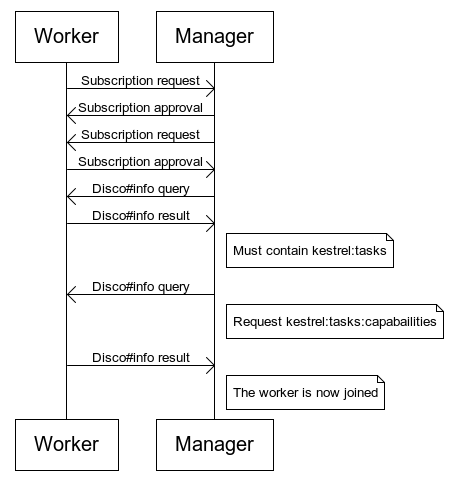
\includegraphics[width=12cm]{figures/join_pool}
\end{centering}
\caption{\label{fig:Joining-the-Pool}The presence subscription and service
discovery process for joining the Kestrel pool. A worker first initiates
a bi-directional presence subscription with the manager, allowing
the manager to know when the worker is available or offline. The manager
then queries the worker's service descriptions to verify that the
agent is a worker, and to find the capabilities the worker provides
that may be used in match making.}
\end{figure}


\begin{lstlisting}[
    label=fig:Discover-Worker,
    caption={Recognizing an XMPP agent as a Kestrel
worker, and discovering its capabilities. The manager first sends
an IQ ``disco'' stanza to the agent; the agent's response must
include the \texttt{kestrel:tasks} feature in order to be accepted
as a worker. Once the worker has been recognized, a second ``disco''
query is issued, this time to the \texttt{kestrel:tasks:capabilities}
node of the agent's profile. The resulting list of features are the
capabilities that the worker offers for use during match making.}
]
<iq to="worker21@example.org" type="get">
  <query xmlns="http://jabber.org/protocol/disco#info" />
</iq>
<iq from="worker21@example.org" type="result">
  <query xmlns="http://jabber.org/protocol/disco#info"> 
    <feature>kestrel:tasks</feature> 
  </query> 
</iq>
<iq to="worker21@example.org" type="get"> 
  <query xmlns="http://jabber.org/protocol/disco#info" 
         node="kestrel:tasks:capabilities" /> 
</iq>
<iq from="worker21@example.org" type="result">
  <query xmlns="http://jabber.org/protocol/disco#info">
    <feature>Python2.6</feature>
    <feature>Linux</feature>
  </query>
</iq>
\end{lstlisting}

\subsection{Task Execution}

\label{sec:Kestrel:Execution} The actual programs executed by workers
should typically be small shell scripts that manages the task's execution
cycle, such as downloading input data and uploading any output. These
scripts will always receive a \textit{final} parameter which is the
task's ID value; however, additional parameters may be passed when
submitting the job by including them with the job's command. The task
ID may also be used as a switch to run different applications with
a single job. Since Kestrel workers are assumed to be behind a NAT
boundary, tasks must operate in a pull model; interactions with external
entities must be done through requests starting from the worker node.

Most applications using Kestrel will need to transfer input data to
the worker and then transfer output data to the user in some fashion.
Some scheduler and dispatch systems, such as Condor, provide built-in
methods for data transfer; however, Kestrel currently does not. While
data transfers may be included in a future release using XMPP's file
sharing capabilities, \texttt{wget} and similar command line utilities
are recommended for now. Transferring files is a largely solved problem
with scalable solutions. The suggested method is to run a HTTP server
(or server cluster) to distribute input files. The HTTP protocol supports
range queries to retrieve sections of a file if needed. A simple upload
form processor may be used to handle receiving output data from workers.

Once a task's command has been executed, an optional second command
may be executed for cleanup purposes. For most cases, this cleanup
script will simply restart the VM to reset its state and release any
disk space used by copy-on-write instances. The cleanup command is
split from the main task command so that if the worker VM is restarted,
the task will not be rescheduled when the manager is notified that
the worker has disconnected while running a task.

\begin{lstlisting}[
    label=fig:Job-Stanza,
    caption={A job submission stanza with two requirements.
The\texttt{ queue} attribute specifies the number of times that the
job will be executed, where each instance is considered a single {}``task''.
Various \texttt{requires} elements may be added to limit set of workers
that may run the job's tasks. When using Kestrel to manage a single
pool shared by various organizations, the organization's identity
is usually added as a requirement so that the job will run on the
organization's VMs.}
]
<iq type="set" to="manager.example.org"> 
  <job xmlns="kestrel:job" action="submit" queue="50000"> 
    <command>/runtask.sh</command> 
    <cleanup>/cleanfiles.sh</cleanup> 
    <requires>Python2.6</requires> 
    <requires>SleekXMPP</requires> 
  </job> 
</iq>
\end{lstlisting}


\begin{figure}
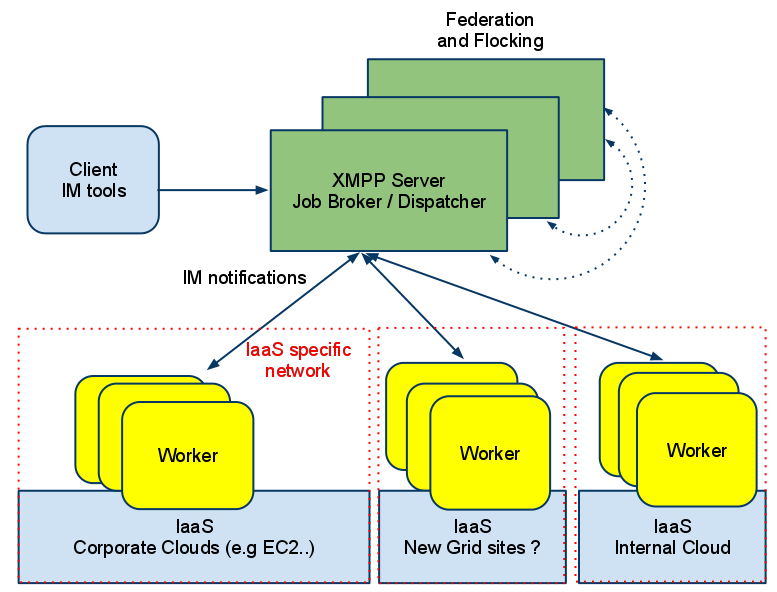
\includegraphics[width=\columnwidth]{figures/kestrel_arch}
\caption{\label{fig:Kestrel-Arch} Kestrel builds a scheduling overlay on top
of Cloud providers. Virtual machines instances containing the Kestrel
worker agent can be started on any Cloud provider using multiple provisioning
systems. Once started the instances join the Kestrel pool irrespective
of the networking setup used by each provider. The Kestrel agents
initiate the connection and setup a instant messaging channel to receive
tasks. The Kestrel manager can make use of the XMPP federation capabilities
to build a scalable pool and establish flocking mechanisms.}
\end{figure}


\section{Manager}
The Kestrel manager is an XMPP component in order to scale to handle
several thousand worker agents \cite{Moffitt2008}. Manager instances
are typically run on the same machine as the XMPP server, but could
also be placed in a VM in a cluster alongside the worker VMs. While
the current backend for the manager is a SQLite \cite{SQLite} database
which can not be shared easily by multiple processes, using a larger
database or a hash value store such as Redis \cite{Redis} would allow
multiple manager instances on different machines to service a single
XMPP server, using the common backend to maintain consistent state.
Such an arrangement would create a clustered manager that still acts
as a single, logical manager instance. However, current research is
focused on manager federation such that Kestrel managers servicing
separate XMPP servers from different organizations may share jobs,
similar to the flocking mechanism in Condor.

\subsection{Scheduling and Dispatching}

\label{sec:Task-Dispatch} Assigning tasks to workers is done
by sending a task IQ stanza to a worker after it has announced its
availability as shown in figure \ref{fig:Task-dispatching}. During
the time period between sending the stanza and receiving a reply,
the task and worker are marked as pending in the manager's internal
data store to prevent assignment conflicts. The current design of
Kestrel limits each worker to accepting only one task instead of multiple
concurrent tasks; the rationale is to simplify matchmaking for the
manager by reducing the number of possible worker states. Future implementations
may remove this limitation. In the event that an error is returned
(as shown in figure \ref{fig:Task-Stanza}), because the worker has
reached its task limit or is no longer online, the task is returned
to the queue to be matched with another worker.

%
\begin{figure}
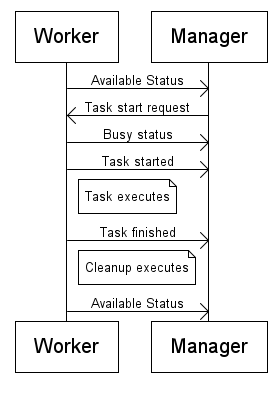
\includegraphics[height=8cm]{figures/dispatch}
\caption{\label{fig:Task-dispatching}The task dispatching and execution process.
A match making request is triggered when the manager receives an available
presence from a worker. If a matching job is found, a task is marked
pending and sent to the worker; if an error is returned or a timeout
occurs, the task is returned to the queue. Otherwise, the worker broadcasts
a busy presence to prevent further job matching, and then notifies
the manager that the task has been started. Once the task's command
has terminated, a finished notice is sent to the manager to mark the
task as completed. An optional cleanup step is then performed before
the worker issues an available presence indicating it is ready for
the next task.}
\end{figure}

As part of the new requirements presented with carrying out the STAR
experiment, a new task attribute was added for carrying out a cleanup
phase. After the main command for a task has been executed, the worker
will report that it has completed the task. However, it will not make
itself available to receive a new task until the cleanup command has
completed, if one has been provided. Such an arrangement allows for
cleanup scripts to shutdown and restart the virtual machine without
causing the manager to treat the shutdown as a network failure and
reassigning the task to another worker.

\begin{lstlisting}[
    label=fig:Task-Stanza,
    caption={A task start stanza and an error reply. Note
the task's ID number is given by the resource identifier of the job's
JID.}
]
<iq type="set" to="worker17@example.org" 
    from="job42@manager.example.org/23">
  <task xmlns="kestrel:task" action="execute"> 
    <command>/runtask.sh</command> 
    <cleanup>/cleanfiles.sh</cleanup>
  </task> 
</iq>
<iq type="error" 
    to="job42@manager.example.org/23" 
    from="worker17@example.org">
  <error xmlns="urn:ietf:params:xml:ns:xmpp-stanzas" 
         type="cancel"> 
    <condition>resource-constraint</condition> 
    <text>The worker is already in use.</text> 
  </error> 
</iq>
\end{lstlisting}

\subsection{Responding to Worker Failures}
Given that it is expected for worker agents to disconnect for various reasons,
whether it be network unreliability or faults in the worker VM itself, the
Kestrel manager must respond gracefully to such outages. These failures
may occur during one of four states:
\begin{enumerate}
\item The worker was idle without any assigned task. In this case, the manager
simply removes the worker from consideration for new tasks.
\item The worker was executing a task. Here a policy must be defined to
determine how to treat the task that was being executed. The approach currently
taken by Kestrel is to discard the current progress of the task and reassign it
to the queue to be executed again. However, it is possible that
the worker's unavailability was caused by a transient network disruption and
that the worker would soon become available again. In situations where such
scenarios are expected to be common, an alternative policy to delay the reassignment
of the task back to the queue may be useful.
\item The worker was executing a task cleanup command. The purpose of the cleanup
command is intended to allow for cases where a VM is restarted to free
disk space on the physical machine. The only actions required by the manager is to
mark the worker as unavailable for future tasks.
\item The worker had been assigned a task, but had not responded to the request. Here
the disconnection occurred during the window between the time the manager issued a 
task request to the worker and the worker's receipt of the request. The task request
itself is timed by the manager so that if a response is not received within ten
seconds the task is inserted back into the queue.
\end{enumerate}

\section{Evolution of the Implementation and Lessons Learned}
\label{sec:Evolution}
During the two years of development, Kestrel underwent significant revisions
to the underlying architecture, each time re-purposing more of the existing
XMPP technologies for the tasks of job scheduling and distribution. Kestrel has
thus moved from simply treating an XMPP connection as a basic socket connection
with a few added features to leveraging several existing protocols to allow
for interroperability with other XMPP agents, service discovery, and using
standard formats for data exchange. As part of this process, the underlying XMPP
library for Python used by Kestrel, SleekXMPP \cite{SleekXMPP}, was improved
and expanded to provide support for the features required by Kestrel; complex
functionality unrelated to job distribution has migrated down to the library
level, such as advanced support for dynamic handling of service discovery
requests and external storage for component rosters.

\subsection{JSON over XMPP Message Stanzas}
The original architecture called for using JavaScript Object Notation (JSON)
\cite{Crockford} to encode application specific information and to then use XMPP
message stanzas to carry the information between the manager and worker agents
in the Kestrel pool. Figure \ref{fig:JSON-message} shows an example of a basic
job submission under this model. The main advantage of this method was that few
changes in infrastructure were required. Common XMPP client programs such as
GTalk or Pidgin could send JSON formatted messages directly, and support for
parsing the JSON messages already existed as part of a class project that served
as the precursor to the Kestrel project (under the same name).While workable,
the design had several disadvantages that necessitated changes during the summer
of 2010 STAR experiment.

\begin{figure}
\begin{lstlisting}[
    caption={[A JSON formatted job submission message]}
]
{"type": "submit",
 "command": "./run_program.sh",
 "cleanup": "./restart_vm.sh",
 "requirements": ["Python", "STAR"],
 "queue": 1000}
\end{lstlisting}
\label{fig:JSON-message}
\caption{A JSON formatted message used in the initial versions of Kestrel for
submitting a command and cleanup task; in this case the commands \texttt{./run\_program.sh}
and \texttt{./restart\_vm.sh}. The requirements that a worker agent had to meet in order
to accept the task are given by the list containing \texttt{Python} and \texttt{STAR}.
To indicate that multiple copies of the command should be executed, the \texttt{queue}
parameter was supplied with the value 1000. The initial \texttt{type} value included
in the message was used for routing the message to the proper message handler.}
\end{figure}

The first disadvantage was that combining JSON data with XMPP is an unnecessary
step that adds overhead, both in terms of parsing time and the increase
in complexity from managing two data formats. The XMPP Design Guidelines \cite{XEP-0134}
provided by the XSF \cite{XSF} dictates that XML should be used for any sub-protocol
implemented on top of XMPP for this reason.

The second shortcoming, the cause of several performance and stability issues, was
the reliance on normal XMPP message stanzas for all communications between agents in
the pool. XMPP message stanzas do not provide strong guarantees of delivery with 
standard server installations; rather, they are treated as ``fire and forget'' payloads
\cite{RFC3921} with no expectation of a response in receipt. Ensuring consistency
between Kestrel's central manager's view of the state of the worker pool, in particular
those workers with pending jobs, and the actual state of the pool became difficult with
large numbers of workers over an extended period of time.

\subsection{Customized IQ Stanzas}
\label{sec:Custom-IQ}
To resolve the deficiencies of the JSON over message stanza model, the
communication channels were moved to use custom XML payloads in IQ stanzas.
The main benefit of this model was the guaranteed response for any IQ stanza
sent. In the case of the recipient disconnecting while the IQ is broadcast,
the XMPP server itself will respond with an error IQ stanza on behalf of the
disconnected agent. In addition, the SleekXMPP library provides a built-in
mechanism for blocking execution while waiting for an IQ response, with an
optional timeout value to handle cases where the recipient received the IQ from
the server, but does not respond. In addition, in conjunction the customized
XML payload, the protocols described in sections \ref{sec:Task-Dispatch} and
\ref{sec:Job-Management} were developed to manage the various work-flows
required to dispatch tasks and manage jobs. As a final improvement, a SQLite
\cite{SQLite} database was used to store all application state using SQLAlchemy
\cite{SQLAlchemy}. A limitation of SQLAlchemy with SQLite was only a single
thread may access the database. All operations touching the database were
therefore serialized, which introduced delays in initializing the pool when
large numbers of workers contacted the manager at once.
